%!TEX root = ../thesis.tex

\chapter{Understanding ASR System}    % (fold)
\label{cha:asr}

Automatic Speech Recognition or ASR is a very active research area since the last five decades \cite{yu_automatic_2015} being an essential medium for Human-Computer Interaction (HCI). Speech Recognition is more than just Physics, Mathematics, and Computer Science (Artificial Intelligence).
\par
In this chapter we will discuss basic concepts as well as nuts and bolts of the ASR system. We will discuss Linguistic and Technology Aspects of Speech Recognition Systems.  

\section{Linguistic Aspects of Speech}
\label{sec:linguistic_aspects_of_speech}

\par
Linguistics is the most important component that gives Speech Technology its structure. Spoken and signed data is considered to be more fundamental than written data by linguists since speech is universal to all humans who are capable of producing and perceiving it. Speech evolved before writing was invented because humans learn and understand speech easier and earlier than learning to read and write \cite{backstrom_introduction_2022}.
\par
Many cultures and speech communities do not have methods for written communication but have linguistic structure in their spoken language. Features like sound changes, phonological rules and speech errors appear in spoken but are not always recorded in written language. All natural systems of writing reflect a spoken or potentially a signed language. The text in writing systems used for two languages changing to fit the spoken language being recorded (e.g. Arabic script to write in Arabic, Farsi, Urdu, Sindhi and in our case using roman script for Urdu and English both) and Pictographic scripts (like Dongba writing Naxi homophones) with the same pictogram reflect spoken language.
\par
Despite this linguists agree on importance of studying written language and its systems referred to as \textit{graphemics}, which is a branch of linguistics. Written language is more effective and convenient to process large amounts of linguistic data in research relying on corpus and computational linguistics. Large Spoken language corpora, usually transcribed and written, are difficult to create and difficult to find.

\subsection{Types of Linguistic Study}
There are two major fields of Linguistic Study \cite{juang_automatic_2005}.

\begin{enumerate}
\item \textbf{Corpus linguistics}, also known as corpus-based studies is the study of language based on large collections of "real life" language use stored in corpora which are computerised databases created for linguistic research e.g. British National Corpus. Sub-language Corpora contains texts sampled from a particular language variety e.g. from a particular dialect or from a particular subject area. 

\item \textbf{Computational linguistics} is an interdisciplinary field that studies appropriate computational approaches to linguistic questions as well as the computational modelling of natural language. To understand language structurally and develop language models, it employs linguistics, computer science, artificial intelligence, mathematics, logic, philosophy, cognitive science, cognitive psychology, psycho-linguistics, anthropology, and neuroscience, among other disciplines. Even computer programming languages like C, C++, Java etc have a variety of logical and linguistic structures.
\end{enumerate}

\subsection{Study of Linguistics and its Components}
\quad Speech is often known to have double articulation or duality of patterning i.e. meaningful speech units, like words and utterances, comprise of less meaningful units like phones or phonemes, which still highlight various distinctions in meaning. 

\quad Linguistic units and their relative organization are language-dependent at all levels e.g. the choice of phones, syllables, or words used and their sequence in a given sentence or context. There are certain linguistic universals or common tendencies either resultant from restrictions in speech production and perception or due to other shared natural languages characteristics. We can understand speech as a hierarchy of elementary units of increasing timescale \cite{backstrom_introduction_2022}.

\begin{figure}[h!]
    \centering
    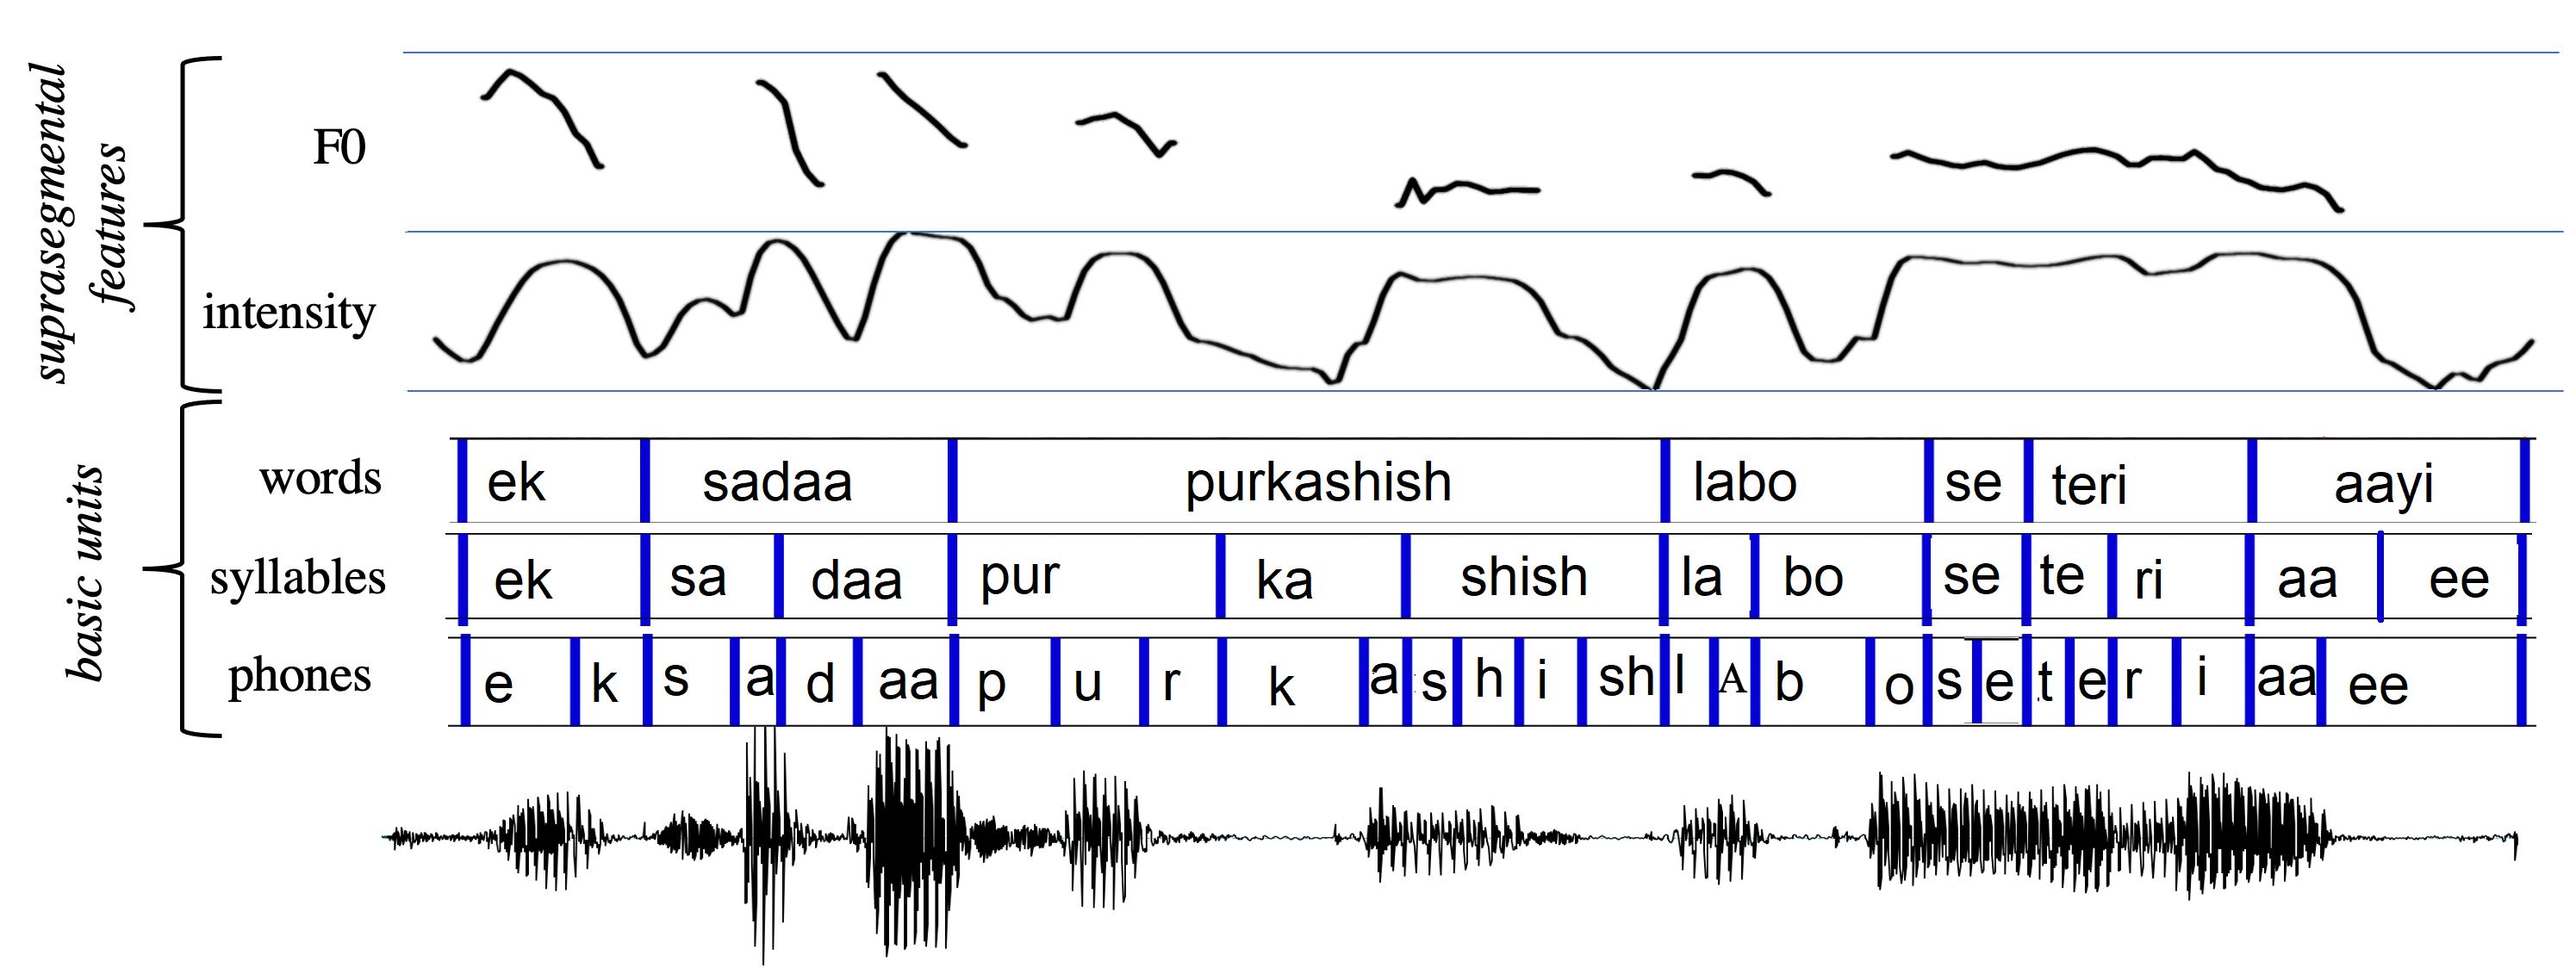
\includegraphics[width=0.9\textwidth]{img/speech3.png}
    \caption{Units of Language}
    \label{fig:units-of-language2}
\end{figure}

Going from lowest to highest units the structure is as follows \cite{brown_encyclopedia_2006}:
\begin{itemize}
    \item \textbf{Phones} are any distinct gesture or speech sound, irrespective of whether the exact sound is essentially required to provide meanings to words. 
    \item \textbf{Phoneme} is a speech sound in a given language that, if swapped with another phoneme could entirely change one word to other. They are the speech sounds that provide us the contrast of meaning between different words. For instance the English word 'cap' has 3 phonemes – 'c' 'a' and 'p'
    \item \textbf{Syllables} are organized sequences of phones. Words are made up of one or more syllables. Syllables are one or more sound sequences consisting of a \textit{syllable-nucleus} which is usually a vowel and an onset (optional initial sequences) and conda (final sound sequences), which tend to have consonant sounds. For instance the English word 'cook' has one syllable, and 'meeting' has two syllables.
    \item \textbf{Words} are the basic units of written and spoken linguistics which contain meaning in isolation as well as in broader context of sentence or a conversation, unlike isolated phones and syllables which carry no meaning on their own except for the cases of monosyllabic words (e.g. hey, Eh). 
    \item \textbf{Utterance} is the smallest un-paused speech production act by single speaker that is preceded by silence and followed by silence or a change of speaker, delineated by speaker change or by clear pauses and it comprises of one or more words. 
    \begin{itemize}
        %\item An utterance is a stretch of spoken language that is preceded by silence and followed by silence or a change of speaker. 
        \item Segments of the stream of speech sounds that make up an utterance are phonemes, morphemes, and words.
        \item  In spoken language utterance tend to differ from single words to longer word streams and grammatical constructs.
        \item Speech, unlike written language, consists of speaking acts of variable duration rather than clearly delineated clauses or sentences. %In contrast to written language, where a sentence is one grammatical expression with a communicated meaning, speech consists of speaking acts of variable duration rather than clearly delineated clauses or sentences.
        \item Speakers tend to use fillers, prolonged vowels, hesitations and filled pauses like “eh” or “umm” or "ah" or "err" to signal their intention continuation of their utterance, but require little time to re-organize their thoughts to formulate the subsequent speech in their mind.
        \item Some examples include saying "150" in math class to answer your teacher's question, Policeman yelling "Stop!", saying "Good boy!" to your pet dog, and even a long one hour speech by the President of a country.      
    \end{itemize}
     \item \textbf{Sentences} - Group of words that follow a coherent structure (syntax), following certain protocols (grammar) is called sentences that contain information and meaning (pragmatics).
\end{itemize}

Aside from the units of speech mentioned above, there are several other units and structural linguistic concepts used in linguistic theory that are less commonly used in speech processing. They do, however, come into play when mapping speech to written language or vice versa, or when using speech processing tools for linguistic research. An example of this type of area of linguistics study is called \textit{morphology} \cite{backstrom_introduction_2022}. 

\section{Speech Features Extraction Process}

Speech Features like frequency, amplitude, resonance, harmonics, pitch, tone etc as a whole can be holistically understood by humans but computers cannot understand them directly. Hence, we need to convert analogue speech signal to Digital. In Digital these nuanced information like frequencies, amplitude etc need to be in an understandable format for the computer. These dimensions need to be broken down in presentable form to make it easy for us to understand and work as well. 

\subsection{Audio Features}
Audio features can be categorized into following:
\begin{enumerate}
    \item High-Level Audio Features keys, chords, rhythm, melody, tempo, lyrics, genre, and mood.
    \item Mid-Level Audio Features include pitch and beat level attributes like MFCCs, Fbanks, CMVN, HEQ, note fluctuation patterns or the start of a musical note called note onsets.
    \item Low-Level Audio Features are generally the statistical features that get extracted from the audio which include amplitude envelope, energy, zero-crossing rate etc. 
\end{enumerate}

There are two main feature extraction and representation processes popularly used:
\begin{enumerate}
    \item Mel-Filter Banks
    \item Mel Frequency Cepstral Coefficients
\end{enumerate}

There is an ongoing debate in the ASR community about using the DCT instead of the log Mel fiter-bank features, especially for Deep Neural Network-based acoustic models \cite{raj_note_nodate}. Filter banks and MFCCs computation is done by almost same procedure; MFCC is calculated after a Cosine Transformation of FilterBanks.

\subsection{Mel-Filter Banks}

The signal goes through following steps to calculate Filter banks after Analogue to Digital Conversion \cite{backstrom_introduction_2022}: 
\begin{enumerate}
    \item Pre-emphasis filter.
    \item Signal Slicing into overlapping frames.
    \item Applying window function to each frame.
    \item Short-Time Fourier Transform or simply Fourier Transform on each frame for power spectrum calculation.
    \item Computation of filter banks. 
\end{enumerate}

Individual frequencies are difficult to distinguish in the raw power spectrum, especially at high frequencies.  To solve this, the spectrum is convolved with several (20-40, in general) triangular Mel filters, referred to as a filterbank, which is wider at higher frequencies because humans do not perceive loudness on a linear scale i.e. at higher the frequency, lower the perceived loudness. Thus these filters are narrow at low frequencies and widen as frequency increases \cite{raj_note_nodate}. The logarithmic scale of Mel-filterbank output is used to reduce the number of acoustic variants that are unimportant for speech recognition. 

Mel scale can be converted from frequency by following formula: \cite{backstrom_introduction_2022}:
\begin{equation}
    M(f)=1125\ln_(1+\frac{f}{400}) \\
\end{equation}
to go from Mels back to Frequency: \\
\begin{equation}
    M^{-1}(m)=700(exp(\frac{m}{125})-1) \\
\end{equation}

\subsection{Mel Frequency Cepstral Coefficient}

MFCC is the industry standard due to its good performance ever since Davis and Mermelstein developed MFCC in the 1980s. It can extract important information from speech signal and audio which is an active research area \cite{noauthor_mfcc_nodate}. 

Since filter-bank energies cannot be used directly with a Gaussian mixture with diagonal covariance and are correlated, they are de-correlated using DCT which is applied to the FBanks to retain a number of the resulting co-efficients while the rest are discarded to compute MFCCs. Mean normalization is applied after this by subtracting the mean of each coefficient from all frames, to balance the spectrum and improve SNR. 

\begin{figure}[h]
    \centering
    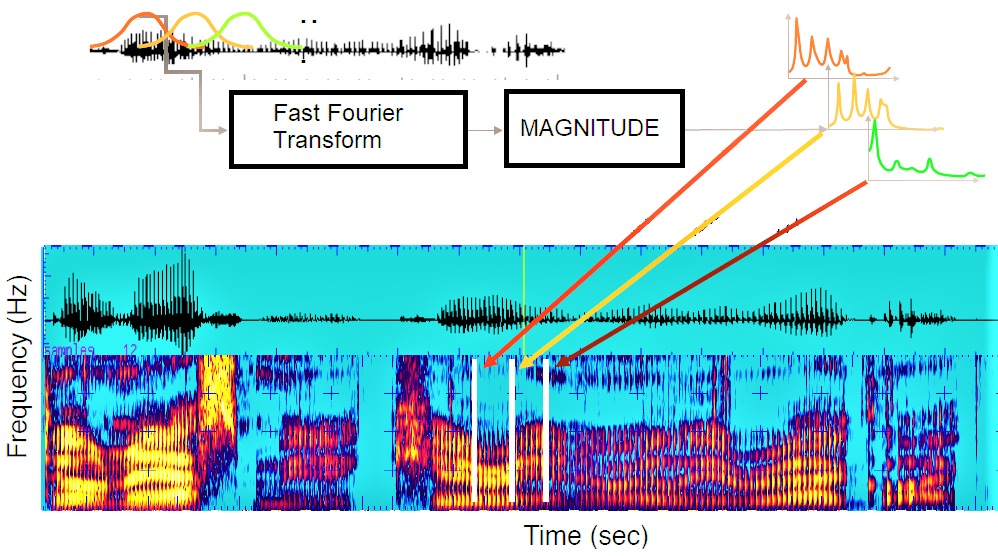
\includegraphics[width=0.8\textwidth]{img/feature extraction22.png}
    \caption{Feature Extraction Pictorial Representation}
    \label{fig:Feature-extraction-pic}
\end{figure}

%Some research groups, such as Google, use filter-banks (fbanks) \cite{noauthor_mfcc_nodate}. 

\begin{figure}[htb]
    \centering
    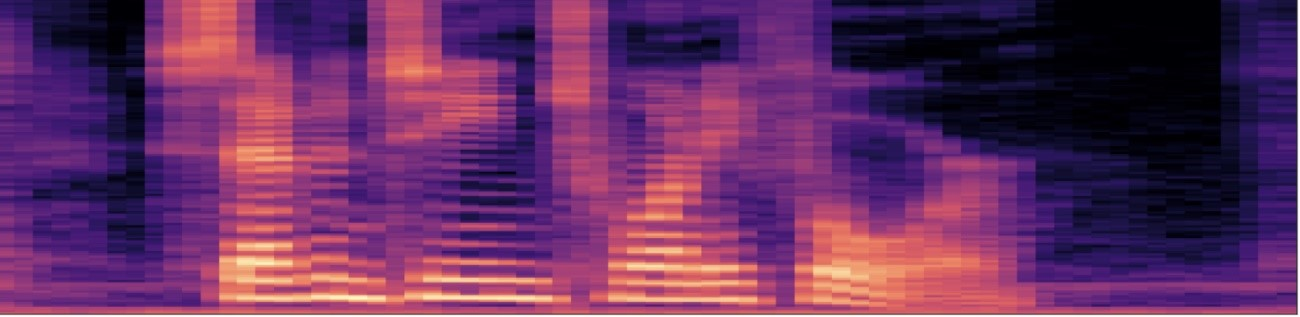
\includegraphics[width=0.7\textwidth]{img/mfcc4.jpg}
    \caption{MFCC - X axis represents time and Y Axis represents features}
    \label{fig:mfcc-example}
\end{figure}

\subsection{Comparing Mel FilterBanks and MFCCs}

The nature and human perception of the speech signal inspired all of the steps required to compute filter banks. The limitations in some ML algorithms  requirement of extra steps in MFCC computation. To de-correlate filter-bank coefficients, DCT is required. This process is also called whitening. MFCCs were popular when HMM-GMM were popular and they co-evolved to be the Standard ASR methods up till late 90s \cite{backstrom_introduction_2022}. 

However, with advancement of NNs and Deep Learning in ASR, Filterbank popularity increased because DNNs are less susceptible to highly correlated input which is why DCT was no longer required \cite{raj_note_nodate}. DCT  being linear transformation discards some information in speech signals which are highly non-linear and hence is considered undesirable \cite{fayek_speech_2016}.

It might be beneficial to attempt to learn directly from the signal in the time domain which has given promising results and bypass Fourier Transform since it is a linear operation and is a difficult operation to learn which may increase data and model complexity required for achievement of same performance. Signal is assumed to be stationary within this short time-frame when doing STFT, which is why the Fourier transform linearity does not pose much of a problem \cite{fayek_speech_2016}.

\section{How Does Computer Understand Speech?}
\label{sec:what-is-asr}

Automatic Speech Recognition refers to the technology that enables communication and interaction with computers using Speech \cite{lakshmi_sri_kaldi_2020}. Humans use their mouth, tongue, lips lungs and larynx to generate sound (emitter) and their ears capture the sound (receiver) which is then captured in the brain, analyzed, understood, and is then processed as thoughts or action. The computer however captures speech sound or audio using a microphone (receiver) and converts the analog signal of speech sound into digital audio so the computer can understand it by creation of a wave file of the spoken words and breaking down of these filtered wave files into phonemes \cite{backstrom_introduction_2022}. 

ASR systems generate the most likely word sequence from a given speech signal. ASR research was dominated by the statistical approach which gave good results. The speech recognition problem statement can be generally defined as \textit{"the conversion of spoken utterances into textual sentences by a machine"}. Bayesian decision rule is employed in this statistical traditional framework to produce the most likely word-sequence given the observation-sequence $O=(o_{1},o_{2}...o_{T})$ \cite{maglogiannis__2020}:

\begin{equation}
\centering
\hat{H} = \argmax_{H} P(H|O)    
\end{equation}

In accordance with Bayes' rule, posterior probability in the above-mentioned equation is expressed as \textit{"product of a conditional probability of the word-sequence given the acoustic observations i.e. P (O|H) and a prior probability of the sequence of words i.e. P (H), and normalised by the marginal likelihood of sequence of observations i.e. P (O)"} \cite{backstrom_introduction_2022}:

\begin{equation}
\centering
\hat{H} = \frac{\argmax_{H} P(O|H) P(H)} {P(O)}
= \argmax_{H} P(O|H) P(H) 
\end{equation}

The marginal probability i.e. P(O) in second equation is omitted because it is constant w.r.t the ranking of hypotheses and thus has no effect on the search for the best hypothesis. The acoustic model calculates P(O|H), while the language model models P(H) \cite{backstrom_introduction_2022}.

\section{Components of Automatic Speech Recognition System}
\label{sec:components-of-asr}

\begin{figure}
    \centering
    %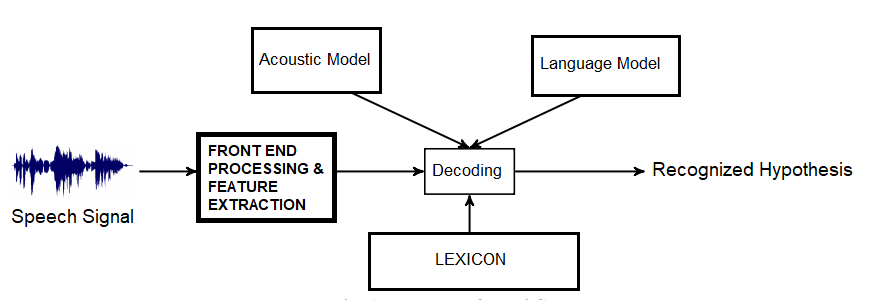
\includegraphics[width=0.8\textwidth]{img/ASR-diagram2.png}
    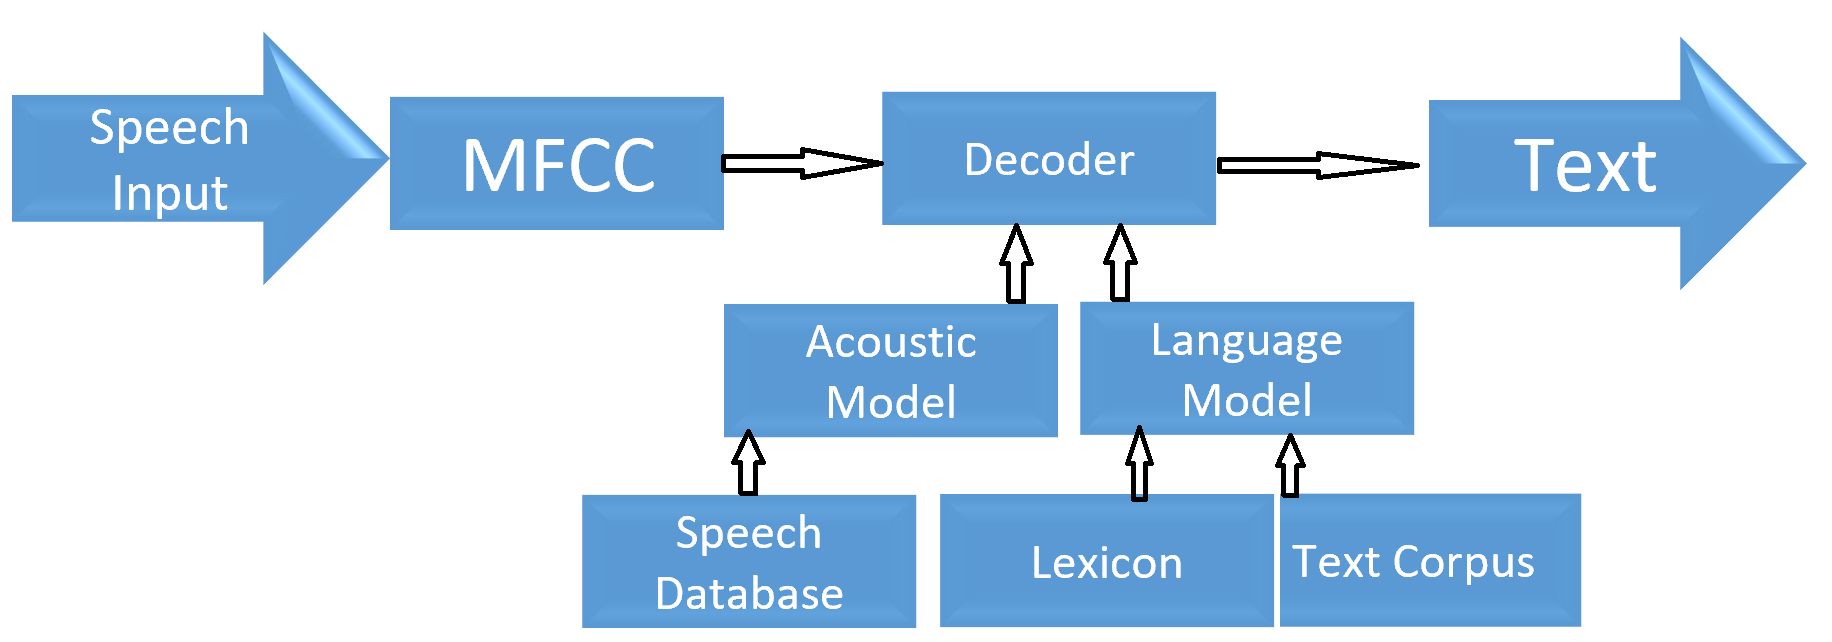
\includegraphics[width=0.7\textwidth]{img/traditional.png}
    \caption{Basic Traditional ASR Architecture}
    \label{fig:asr-diag-arch}
\end{figure}

%\begin{figure}[h]
%    \centering
%    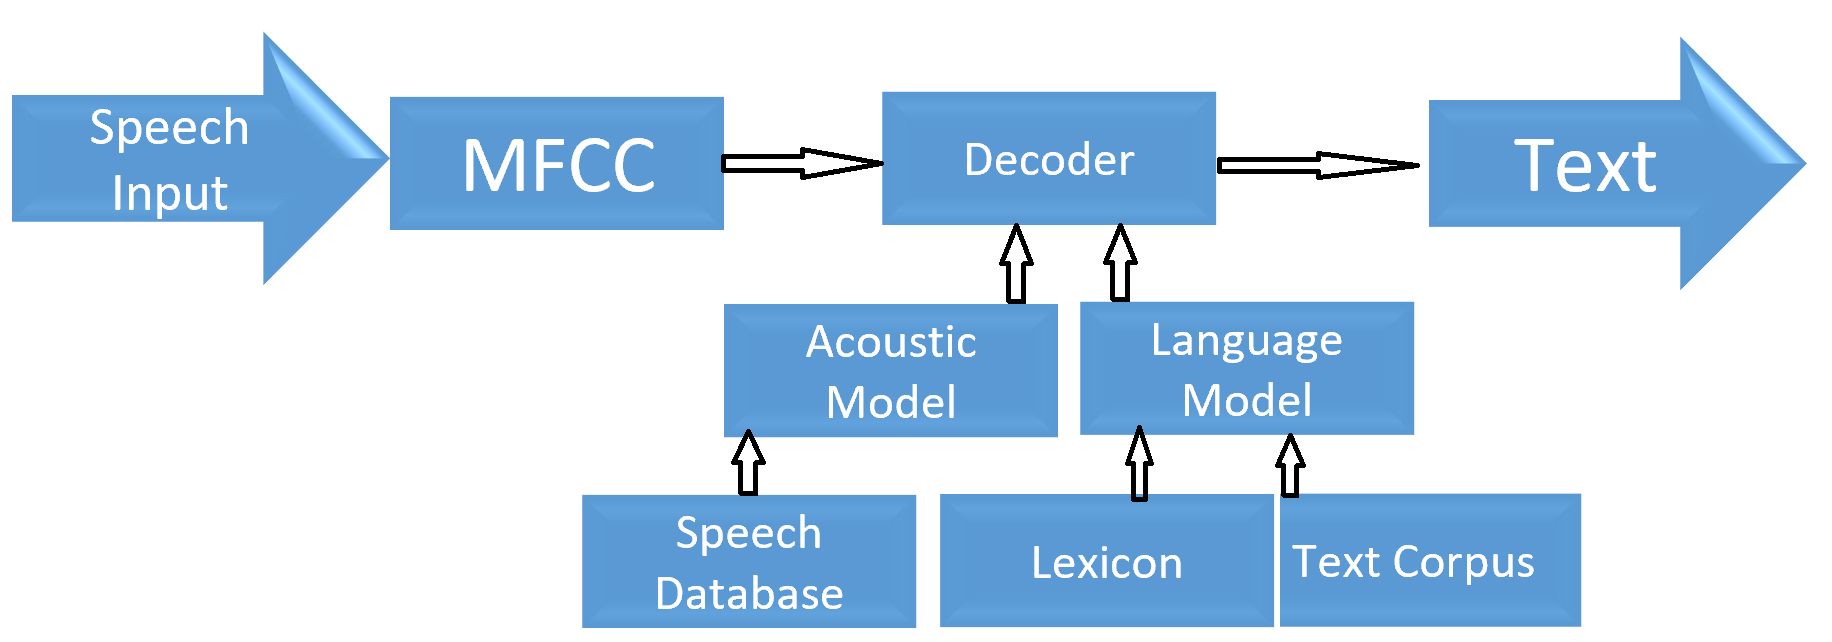
\includegraphics[width=0.7\textwidth]{img/traditional.png}
%    \caption{Traditional ASR}
%    \label{fig:trad-asr}
%\end{figure}

An ASR application takes speech signal input to convert it into a sequence of words in text form as output. During the speech recognition process, a list of possible texts is generated, and the most relevant text to the original sound signal is selected \cite{davis_automatic_1952}. The basic ASR system architecture is given in Figure \ref{fig:asr-diag-arch}.

The vocabulary of ASRs increased to 1000s of words from a few hundred in the 1980s thanks to a new statistical method called "Hidden Markov Model (HMM)," which estimated the probability of unknown sounds actually being words rather than just using words and looking for sound patterns \cite{suma_swamy_evolution_2013}. For a long time, the HMM-GMM was regarded as the standard model for large vocabulary continuous speech recognition (LVCSR), producing the best results.

Statistical models give better performance on low-resource languages with speech data of around 10-30 hours \cite{naeem_subspace_2020}. They offer a strong mathematical foundation, effective learning and decoding techniques, good sequence abstractions, temporal aspects, and flexible topology for statistical phonology and syntax \cite{morgan_continuous_1995} %They provide a Rich mathematical framework, Powerful learning and decoding methods,good abstractions for sequences, temporal aspects and flexible topology for statistical phonology and syntax.

In general ASR systems have following main components \cite{maglogiannis__2020}:

\begin{enumerate}
    \item \textbf{Front End:} Here the speech signal is accepted as input and is sent to relevant modules to extract useful features\cite{s_review_2016}.  
    \item \textbf{Feature Extraction:} The input speech signal is converted into a sequence of acoustic feature vectors or observations which are compact and contain information for later stages of recognition. Some spectra-temporal analysis of the signal generates features that typically transform into more compact and robust vectors %Common feature vectors include Principle Component Analysis (PCA), Linear Discriminant Analysis (LDA), Independent Component Analysis (ICA), Linear Predictive Coding (LPC), Cepstral Analysis, Mel-Frequency Scale Analysis, Filter-Bank Analysis, Mel-Frequency Cepstrum Coefficients (MFCC), Kernel Based Feature Extraction, Dynamic Feature Extraction, Wavelet-based features; Spectral Subtraction and Cepstral Mean Subtraction (CMS) 
    \item \textbf{Language Model:} It contains a lexicon of words and their likelihood of occurrence in a given sequence (in a corpus). It includes terms from the current application's or context's vocabulary. It specifies the constraints associated with the sequence of words accepted in a given language. %Commonly used tools for language modelling are the CMU Statistical Language Modeling (CMU-SLM) Toolkit and the Stanford Research Institute Language Modeling Toolkit (SRILM) \cite{maglogiannis__2020}.      
    \item \textbf{Acoustic Model:} It consists of acoustic features for each distinct phonetic units, referring to the process of establishing the statistical representations for the feature vector sequences computed from the speech waveform i.e. it contains a statistical representation of the distinct sounds forming these words in the grammar or the overall Language Model. Each distinct sound corresponds to a phoneme. The acoustic lexicon and language model are used in the processing stage by a search algorithm or decoder to produce the hypothesised phoneme or word. %The Commonly used Acoustic Modelling methods are Hidden Markov Models, Segmental Models, Super Segmental Models, Neural Networks (Deep Neural Network, Recurrent Neural Networks, Convolutional Neural Network, Time Delay Neural Network and CNN-TDNN), Maximum Entropy Models and Conditional Random Field.    
    \item \textbf{Decoder:} This software searches the acoustic Model for equivalent sounds to the sounds spoken by a speaker. The decoder determines the phoneme associated with that sound when a match is discovered. It keeps track of the phonemes that match until there is a pause in the speaker's speech. The language model is then searched for the equivalent phoneme series or sequence. It gives the text of the corresponding word or phrase as output when a match is found. The decoder tries to find the most likely sequences of words matching the audio signal by applying appropriate models. Most commonly, decoder algorithms produce the \textit{n-best list} which is the list of possible sequence of words. 
\end{enumerate}    
For Scoring and Evaluation, we use string edit distance to determine how accurate our speech recognizer is. To align ASR output with reference transcription, we use dynamic programming. Insertion, deletion, and substitution are the three types of errors and one way to address these types of errors are by calculating WER. If reference transcripts contain N words and ASR output contains "S" substitutions, "D" deletions, and "I" insertions, then \cite{morris_wer_2004}:

   \begin{equation}
       WER = 100.\frac{W+D+I}{N} \% \quad \quad Accuracy = 1-WER \%
   \end{equation} 

ASR engines have their own scoring scripts which compare its transcription with the ones provided by users as references and scores it as Word and Sentence Error Rates. Release of new test sets based on common training and development data on which different systems can be evaluated using WER. A WER of 5\% roughly corresponds to one missed word out of every twenty. If each sentence contains 20 words (which is about average for English), the sentence error rate could reach 100\% \cite{patil_automatic_2016}.

\section{Types of ASR}
\label{sec:types-asr}
In terms of application of ASR systems the types of ASR include \cite{backstrom_introduction_2022}:
\begin{enumerate}
    \item Voice Activity Detection
    \item Speech to Text
    \item Text to Speech
    \item Voice Identification
    \item Speech Enhancement
    \item Speaker Diarization
    \item Wake Word Detection
    \item Para-linguistic Speech Processing and Analysis (Speech Emotion Recognition)
\end{enumerate}

\section{Uses of ASR}
\label{sec:uses-of-asr}
Some common uses of ASR are as follows \cite{backstrom_introduction_2022}:
\begin{itemize}
    \item Quality of Service
    \item Speech Transcription or Dictation services
    \item Call monitoring, transcription and analysis
    \item Speaker identification for secure premises
    \item Subtitle generation for streaming services
    \item Vocalist and Instrument recognition in songs
    \item Medical uses e.g. detecting Alzheimer \cite{konig_automatic_2015}, speech disorders, stress etc.
\end{itemize}





